\documentclass{article}

\usepackage[margin=0.5in]{geometry}
\usepackage[czech]{babel}
\usepackage{graphicx}
\usepackage{booktabs, vwcol}
\usepackage[texMathDollars,pipeTables=true,tableCaptions,hybrid]{markdown}

\begin{document}

\begin{center}
  \Large \bfseries
Model dravce a kořisti
\end{center}
\pagestyle{empty}


Jednoduchý model predace představili nezávisle na sobě A. Lotka a
V. Volterra.

Velikosti populace kořisti a predátora jsou po řadě $x$ a $y$.

Model předpokládá následující.

\begin{itemize}
\item Populace kořisti je daleko pod svou kapacitou prostředí a
  vnitrodruhová konkurence není významná.
\item Každý predátor loví samostatně nezávisle na ostatních. Každý
  predátor loví s konstantním úsilím a uloví poměrnou část kořisti, která je v jeho dosahu.
\item Ulovená kořist se daným procentem projeví příznivě na růstu populace predátora. 
\item Predátor nemá alternativní potravu a bez kořisti vymírá konstantní rychlostí per-capita.
\end{itemize}

\begin{equation*}
\begin{aligned}
\frac{\mathrm dx}{\mathrm dt}={}&ax-bxy\\
\frac{\mathrm dy}{\mathrm dt}={}&-cy+dxy
\end{aligned}
\end{equation*}

\begin{itemize}
\item Nenulovým stacionárním bodem je bod $x=\frac dc$ a $y=\frac
ab$. Velikosti obou populací kolísají okolo tohoto bodu. 
\item Paradoxem je, že velikost populace kořisti kolísá okolo bodu závisejícího na parametrech populace dravce a naopak. 
\item Perioda oscilací závisí na počáteční podmínce.  
\item Přidáním vnitrodruhové konkurence do populace kořisti se systém stabilizuje. 
\item Cykly blízké stacioárnímu bodu mají rfelativně malé oscilace. Výrazným zásahem do populace, například výraznou redukcí populace dravce, se systém dostane na jiný cyklus, kde jsou vysoké výkyvy obou populací. 
  
\end{itemize}


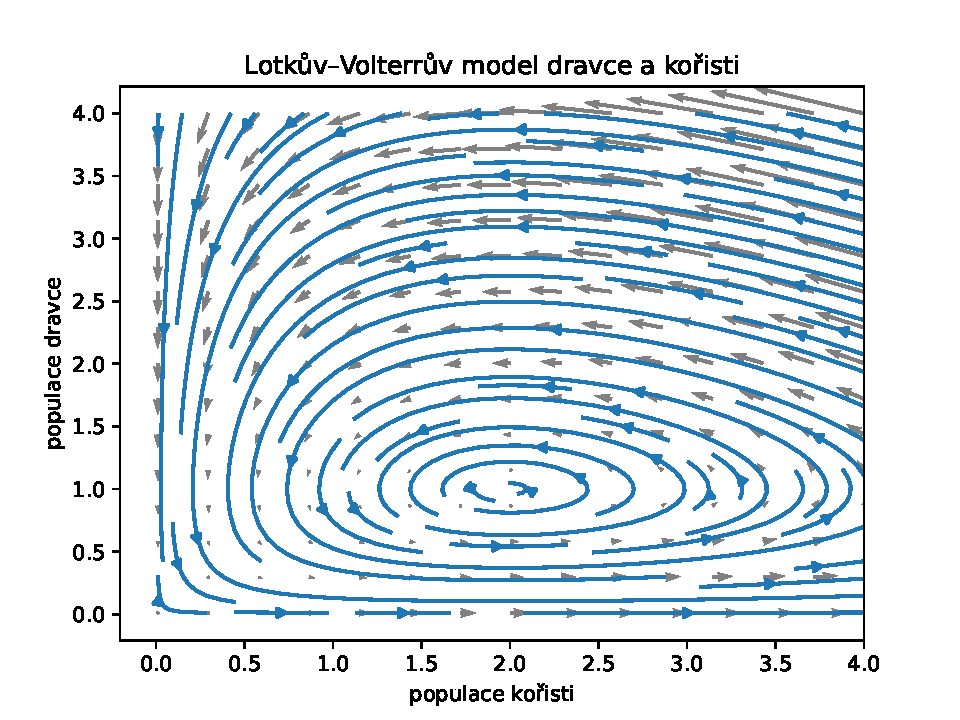
\includegraphics[width=0.5\hsize]{Lotka-Volterra_portret.pdf}
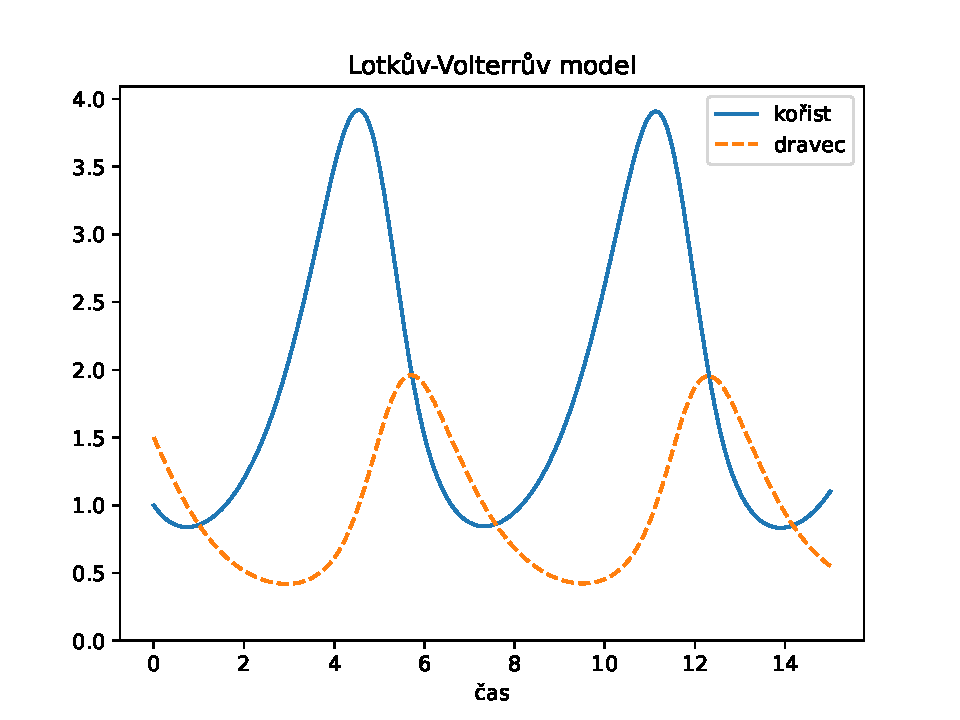
\includegraphics[width=0.5\hsize]{Lotka-Volterra_prubeh.pdf}





\end{document}


%%% Local Variables: 
%%% TeX-command-extra-options: "-shell-escape"
%%% End:
